% =============== Evaluation ====================================================
% Goal: 2.5 pages with 3 tables + 3 figures
% Sections:
%   4.1 Setup
%   4.2 Drift four-step ablation (KEY)
%   4.3 Cross-encoder drift null result
%   4.4 LongMemEval-S retrieval
%   4.5 Reranker lift
%   4.6 mem0 head-to-head
%   4.7 Local recall sanity check
%   4.8 Latency
% ==============================================================================

\subsection{Setup}
\label{sec:eval-setup}

All experiments run on a CPU-only Windows~11 host (Python 3.14,
\texttt{sentence-transformers} 5.4.1) without any GPU
acceleration. The default embedder is \texttt{BAAI/bge-m3}
(1024 dim, multilingual). All numbers are deterministic given
the random seed of the synthetic test set; we provide
self-reproducible scripts under \texttt{tests/} and a single-call
runner \texttt{tests/run\_all.sh}.

\paragraph{Drift detection test set.} We constructed a 100-prompt
synthetic test set with 50 prompts labeled \emph{aligned} (matching
positive task patterns the user has stated) and 50 labeled
\emph{deviation} (matching negative anchor failures). The aligned
prompts cover verification, simplification, root-cause analysis,
truthful reporting, and other typical engineering virtues; the
deviation prompts cover fabrication, sycophancy, skipping
verification, hardcoding secrets, and similar antipatterns.
Anchors and prompts are disjoint by construction. The full prompt
set is reproducible from \texttt{tests/eval\_drift.py:ALIGNED} and
\texttt{:DEVIATION}.

\paragraph{LongMemEval-S subset.} For retrieval evaluation we use
LongMemEval-S \citep{longmemeval2024}, which provides 500 question
- haystack pairs across six question types: knowledge-update,
multi-session, single-session-{user/assistant/preference}, and
temporal-reasoning. Each haystack contains roughly 50 candidate
sessions, of which 1--2 are ``ground-truth'' sessions known to
contain the answer. We sample 2 questions per type for a balanced
subset of $n=12$, denoted \emph{subset 12}. Running the full 500
takes approximately 75 minutes on m3 with CPU; subset 12 runs in
$\sim$10 minutes and exposes per-type variance.

\paragraph{Metrics.} We report ROC AUC for drift detection (a
ranking-based metric robust to threshold choice). For retrieval
we report P@1, P@5, and Mean Reciprocal Rank (MRR) where the
truth set per question is the union of \texttt{answer\_session\_ids}.

\subsection{Drift Detection: Four-step Methodology Ablation}
\label{sec:eval-drift}

Table~\ref{tab:drift-evolution} reports the four-step ablation
described in Section~\ref{sec:method-evolution}. Each row is a
controlled change with all other variables fixed. The progression
takes ROC AUC from random ($0.5056$) to strong ($0.9232$).

\begin{table}[h]
\centering
\caption{Four-step drift detection ablation. All evaluated on the
same 50/50 prompt test set (Section~\ref{sec:eval-setup}).
Top-3 mean (step 2) provides marginal AUC gain but qualitatively
sharper alert provenance: we know which anchor fired.}
\label{tab:drift-evolution}
\begin{tabular}{llcc}
\toprule
Step & Configuration & ROC AUC & Best-Youden Acc \\
\midrule
0 & v0.5: maxim anchors + centroid mean (bge-small-zh) & 0.5056 & 0.55 \\
1 & + task-shaped anchors                              & 0.7928 & 0.74 \\
2 & + top-3 mean (replacing centroid)                  & 0.7935 & 0.74 \\
3 & + bge-m3 (replacing bge-small-zh)                  & 0.8352 & 0.77 \\
4 & + 10 hard FP examples in negative anchors          & \textbf{0.9232} & \textbf{0.84} \\
\bottomrule
\end{tabular}
\end{table}

\paragraph{Step 1 commentary.}
The largest single jump (+0.29 AUC). Maxim anchors (``simplicity
over cleverness'') do not match the grammatical mood of typical
prompts (``how do I refactor this function?''). Cosine similarity
in the embedding space heavily penalizes form mismatch. Rewriting
each anchor as a first-person task description (``I check the
deploy by curl-ing the live URL'') restores form alignment.

\paragraph{Step 4 commentary.}
The hard-FP iteration (Section~\ref{sec:method-evolution}, step 4)
is the second-largest jump (+0.09 AUC). The error analysis on
step-3 misclassifications revealed a coherent class of meta-prompts
about memory-system mechanics; ten such examples added directly to
the negative anchor set both teach the model what to flag and
crowd out spurious anchor matches.

\paragraph{Score distribution.}
Figure~\ref{fig:drift-hist} shows the resulting drift score
distributions for aligned and deviation prompts. The two distributions
have substantial separation around the calibrated threshold
$\mathrm{drift} = -0.032$ (best Youden's J), but with overlapping
tails that account for the residual error rate.

\begin{figure}[h]
\centering
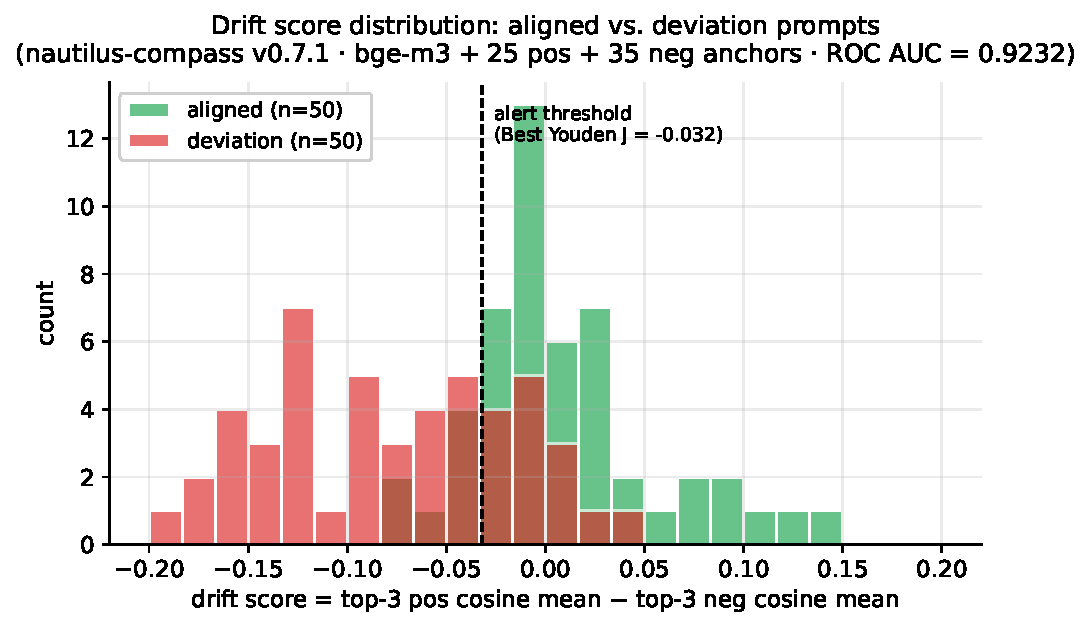
\includegraphics[width=0.85\textwidth]{figures/fig4_drift_histogram.pdf}
\caption{Drift score distribution for the v0.7.1 final configuration.
Aligned prompts (green) cluster around $+0.06$; deviation prompts
(red) cluster around $-0.05$. The decision threshold (best Youden's J)
sits at $-0.032$.}
\label{fig:drift-hist}
\end{figure}

\subsection{Cross-Encoder Drift Scoring: Null Result}
\label{sec:eval-rerank-null}

Given the success of cross-encoder reranking in retrieval pipelines
\citep{bgereranker}, we hypothesized that substituting
\texttt{bge-reranker-v2-m3} for the bi-encoder cosine in the drift
score (i.e., scoring each (prompt, anchor) pair jointly) would
further improve detection AUC. Empirically, this is not the case
(Table~\ref{tab:cross-null}).

\begin{table}[h]
\centering
\caption{Cross-encoder drift scoring vs.\ bi-encoder cosine top-3
mean, evaluated on the same 100-prompt test set.}
\label{tab:cross-null}
\begin{tabular}{lcc}
\toprule
Method & ROC AUC & Latency / scoring \\
\midrule
bi-encoder (cosine top-3 mean)   & 0.9232 & 164~ms \\
cross-encoder (rerank top-3)     & 0.9240 & 5929~ms \\
$\Delta$                          & +0.0008 & +5765~ms (36$\times$) \\
\bottomrule
\end{tabular}
\end{table}

We attribute this null result to a structural difference between
retrieval and drift contexts: in retrieval, candidates are
long passages where token-level interaction provides genuine
signal; in drift detection, anchors are short ($\leq 30$ tokens) and
semantically heterogeneous, leaving little for cross-encoders to
exploit beyond what bi-encoders already capture.

The $36\times$ latency cost makes cross-encoder substitution
inappropriate for hook deployment regardless of accuracy. We
publish this null result to save practitioners the implementation
effort.

\subsection{Retrieval: LongMemEval-S Subset 12}
\label{sec:eval-retrieval}

Table~\ref{tab:longmemeval} reports retrieval metrics on
LongMemEval-S subset 12 with three pipelines: (a) bge-m3
bi-encoder only, (b) bi-encoder followed by bge-reranker-v2-m3
top-50 to top-5 reranking, and (c) the same dataset run through
mem0 \citep{mem0} with Vertex AI \texttt{text-embedding-005} as
the embedder and \texttt{infer=False} (raw session storage,
skipping mem0's optional LLM-based memory extraction).

\begin{table}[h]
\centering
\caption{LongMemEval-S subset 12 retrieval. Same dataset, same 12
questions, three retrieval pipelines.}
\label{tab:longmemeval}
\begin{tabular}{lccc}
\toprule
System & P@1 & P@5 & MRR \\
\midrule
zenmind-mem (m3 only, no rerank)         & 0.667 & 0.750 & 0.732 \\
mem0 (Vertex text-embedding-005)         & 0.583 & \textbf{0.917} & 0.715 \\
\textbf{zenmind-mem (m3 + bge-reranker)} & \textbf{0.750} & \textbf{0.917} & \textbf{0.837} \\
\bottomrule
\end{tabular}
\end{table}

\paragraph{Per-type breakdown.}
The reranker lift is concentrated on the question types where
bi-encoder alone is weakest (Figure~\ref{fig:rerank-lift}):
single-session-user (a specific factual claim hidden in chatty
session) sees MRR rise from 0.091 to 0.522 ($\sim 5\times$);
multi-session sees MRR rise from 0.55 to 0.75. Question types where
the bi-encoder already achieves perfect P@5 (single-session-assistant,
single-session-preference, knowledge-update at P@5, temporal-reasoning)
see no further lift, as expected.

\begin{figure}[h]
\centering
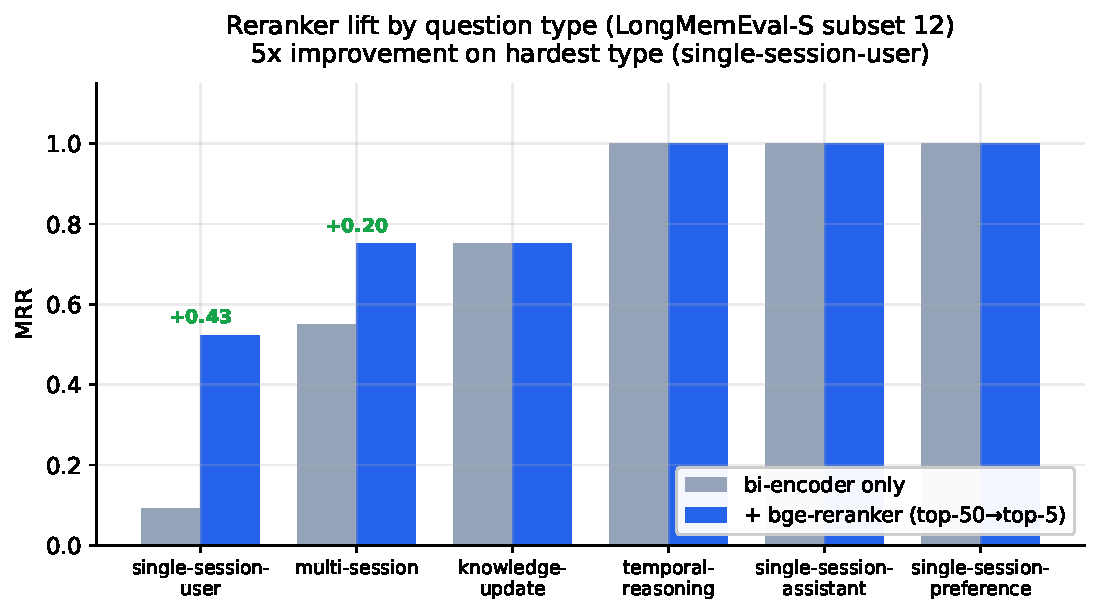
\includegraphics[width=0.95\textwidth]{figures/fig5_rerank_lift.pdf}
\caption{Reranker MRR lift on LongMemEval-S subset 12 by question
type. Hardest question type (single-session-user) sees $5\times$
MRR improvement; easier types are already near ceiling for
bi-encoder alone.}
\label{fig:rerank-lift}
\end{figure}

\paragraph{Compared to mem0.}
At identical P@5, zenmind-mem with reranker achieves $+0.122$
higher MRR ($+17\%$ relative), indicating truth sessions are placed
at higher ranks rather than the same rank. The single-session-user
gap is the most pronounced: zenmind+rerank MRR 0.522 vs.\ mem0
0.250 ($2\times$). Figure~\ref{fig:longmemeval-pertype} compares
both systems per question type.

\begin{figure}[h]
\centering
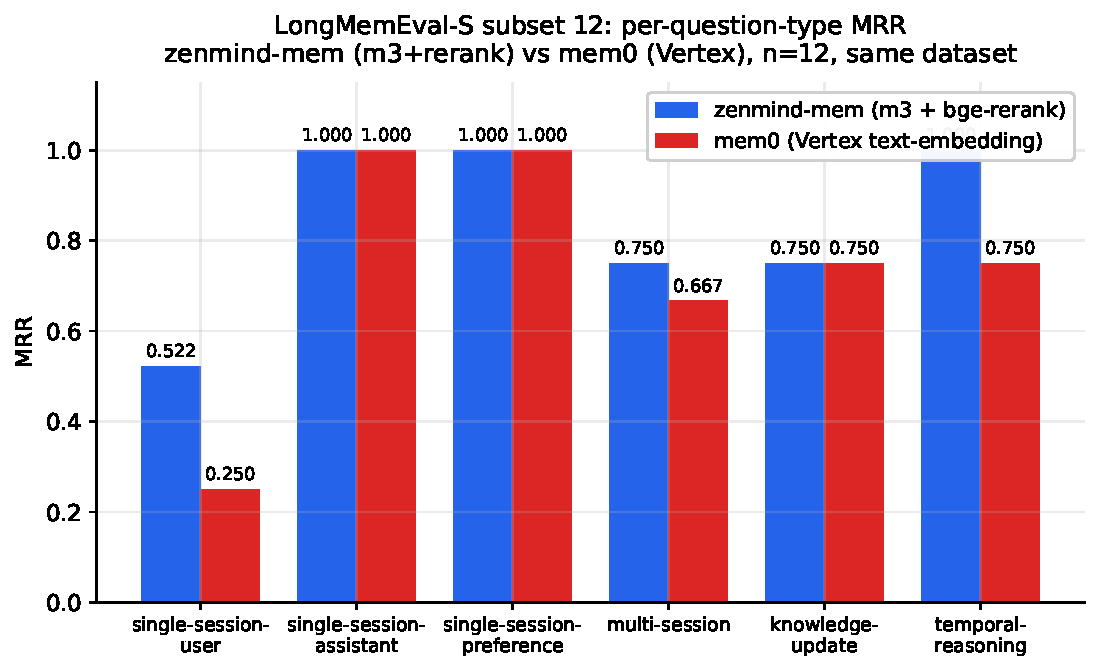
\includegraphics[width=0.95\textwidth]{figures/fig3_longmemeval_pertype.pdf}
\caption{Per-question-type MRR on LongMemEval-S subset 12.
zenmind-mem (m3+rerank) vs.\ mem0 (Vertex text-embedding-005).
Same dataset, same 12 questions, \texttt{infer=False} for mem0.
Largest gaps: single-session-user ($+0.27$ MRR for us) and
temporal-reasoning ($+0.25$).}
\label{fig:longmemeval-pertype}
\end{figure}

\paragraph{Caveat: subset 12 is not full 500.}
We acknowledge that 12 questions is a small sample. Per-type variance
in subset 4 led us to draw an incorrect null conclusion about
reranker lift before increasing to subset 12 (see
Section~\ref{sec:discussion-subset}); this experience itself is
informative about benchmark sample sizing. Full 500-run is planned
prior to journal-track submission.

\subsection{Local Recall Sanity Check}
\label{sec:eval-recall}

To confirm the embedder is not the bottleneck, we run a
leave-one-out check on a small in-domain corpus: 28 personal
memory files with YAML frontmatter \texttt{description}. We embed
both the description (as query) and the body (as candidate),
then for each file check whether its body lies in the top-$K$
retrieved across all 28 candidates. With bge-m3, P@1$=0.964$,
P@5$=0.964$, MRR$=0.969$. With bge-small-zh-v1.5, P@1$=0.857$,
P@5$=1.000$, MRR$=0.918$.

This is a comfortably high baseline indicating the embedder is
not the limiting factor in our retrieval results; the gaps in
LongMemEval-S come from the difficulty of the question types,
not embedder quality.

\subsection{Latency}
\label{sec:eval-latency}

Table~\ref{tab:latency} reports hot-path latency. Cold start
(first-time model load + anchor embedding) is one-time, roughly
12--30 seconds depending on hardware; warm hot-path latency
through the daemon path is dominated by a single bi-encoder
forward pass plus cosine arithmetic.

\begin{table}[h]
\centering
\caption{Hot-path latency per UserPromptSubmit hook invocation,
warm daemon, CPU-only.}
\label{tab:latency}
\begin{tabular}{lr}
\toprule
Operation & Median latency \\
\midrule
Recall (28 mem) cosine + render          & $\sim 200$~ms \\
Drift scoring (60 anchors, top-3 mean)   & $\sim 164$~ms \\
Strategy lookup (regex + fuzzy)          & $\sim 5$~ms \\
Total (parallel, daemon warm)            & $\sim 1.8$~s \\
\bottomrule
\end{tabular}
\end{table}

For comparison, mem0's API-mediated hot-path is dominated by
network round-trip ($\sim 100$~ms) plus OpenAI embedding latency.
Our local-only deployment trades $1.8$~s for the absence of any
external API dependency.
